\documentclass[a4paper]{article}
%\usepackage{graphicx}
\usepackage{amsmath}
\usepackage{svg}

\usepackage{geometry}
 \geometry{
 a4paper,
 total={150mm,257mm},
 top=20mm,
 }

\newcommand{\di}{i}

\begin{document}
\iffalse
Ziel: Zusammenfassung der bisherigen Daten fuer QPC und Half Barrier

Was willst du zeigen?
* QPC mit edge currents (schmaler Spalt an der Seite)
* QPC-like setup, aber nur zwei schmale Spalte an den Seiten
* QPC fuer hoeheres Splitgate

Half Barrier
%* Oberer Finger (check)
%* Unterer Finger (check)
* Rechnung hinzufuegen?

Waveguide

Waveguide mit Gate in der Mitte?

NPN junction? 
\fi

\section{QPC}
\iffalse

Entschieden für decay 20, weil da die Transmissionskurve deutlich früher wieder hochgeht. Gerade laufen Bandstruktur berechnungen, damit kann ich dann sagen, bei welchen Splitgate ich welche dotierung habe.
Wenn das steht, kann ich zeigen, wie das beating pattern verschwindet und wieder auftaucht. 

Dann kann ich mit diesen Parametern die Spalte an den Seiten dazu modellieren und diese Plots mitaufnehmen. 

Arbeitsschritte: 
* Leitfähigkeit für decay 30 (check)
* Vergleiche mit Leitfähigkeit für decay 20 (check) 
* Bandstruktur berechnen (läuft, als nächstes commiten, plotten und einfügen) (check)
* Strom Plots machen: dafür parameter checken und vereinheitlichen!
* Mit den gleichen Parametern das QPC mit Spalten modellieren (check), plotten, welche Daten fehlen?
* Weitere Möglichkeiten: Doping an den Rändern manuell erhöhen?
\fi

\begin{figure}
\centering
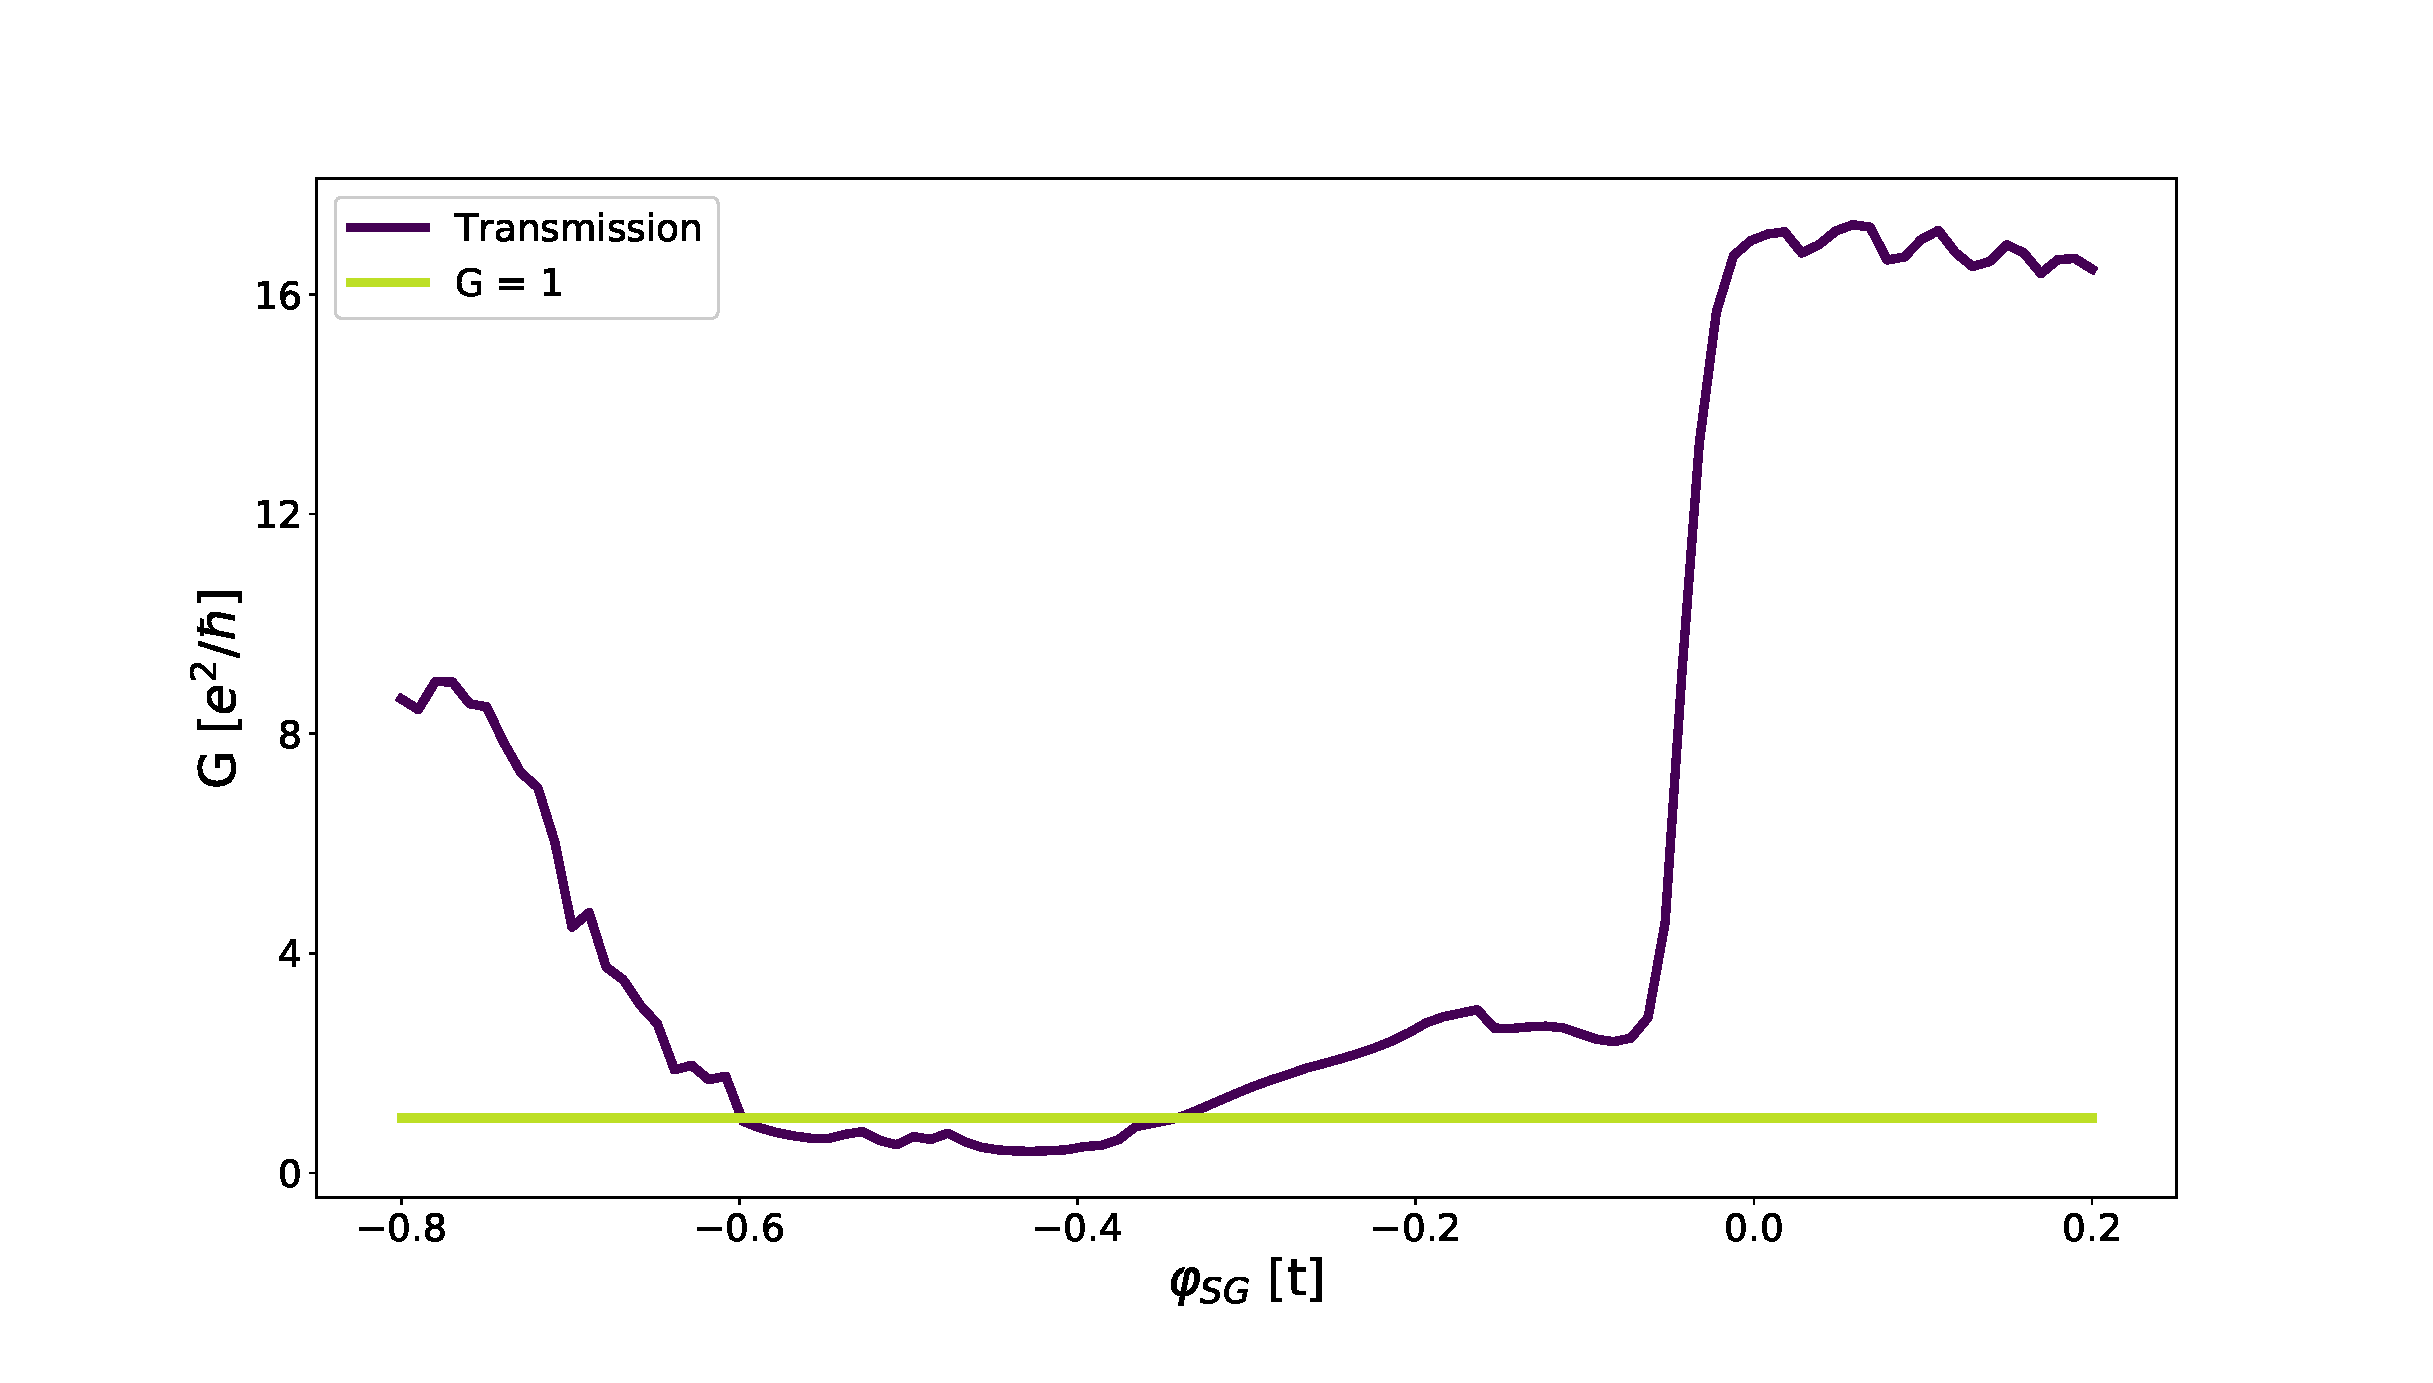
\includegraphics[width=\textwidth]{qpc-conductance}
\caption{Conductance of QPC setup}
\end{figure}

\begin{figure}
\centering
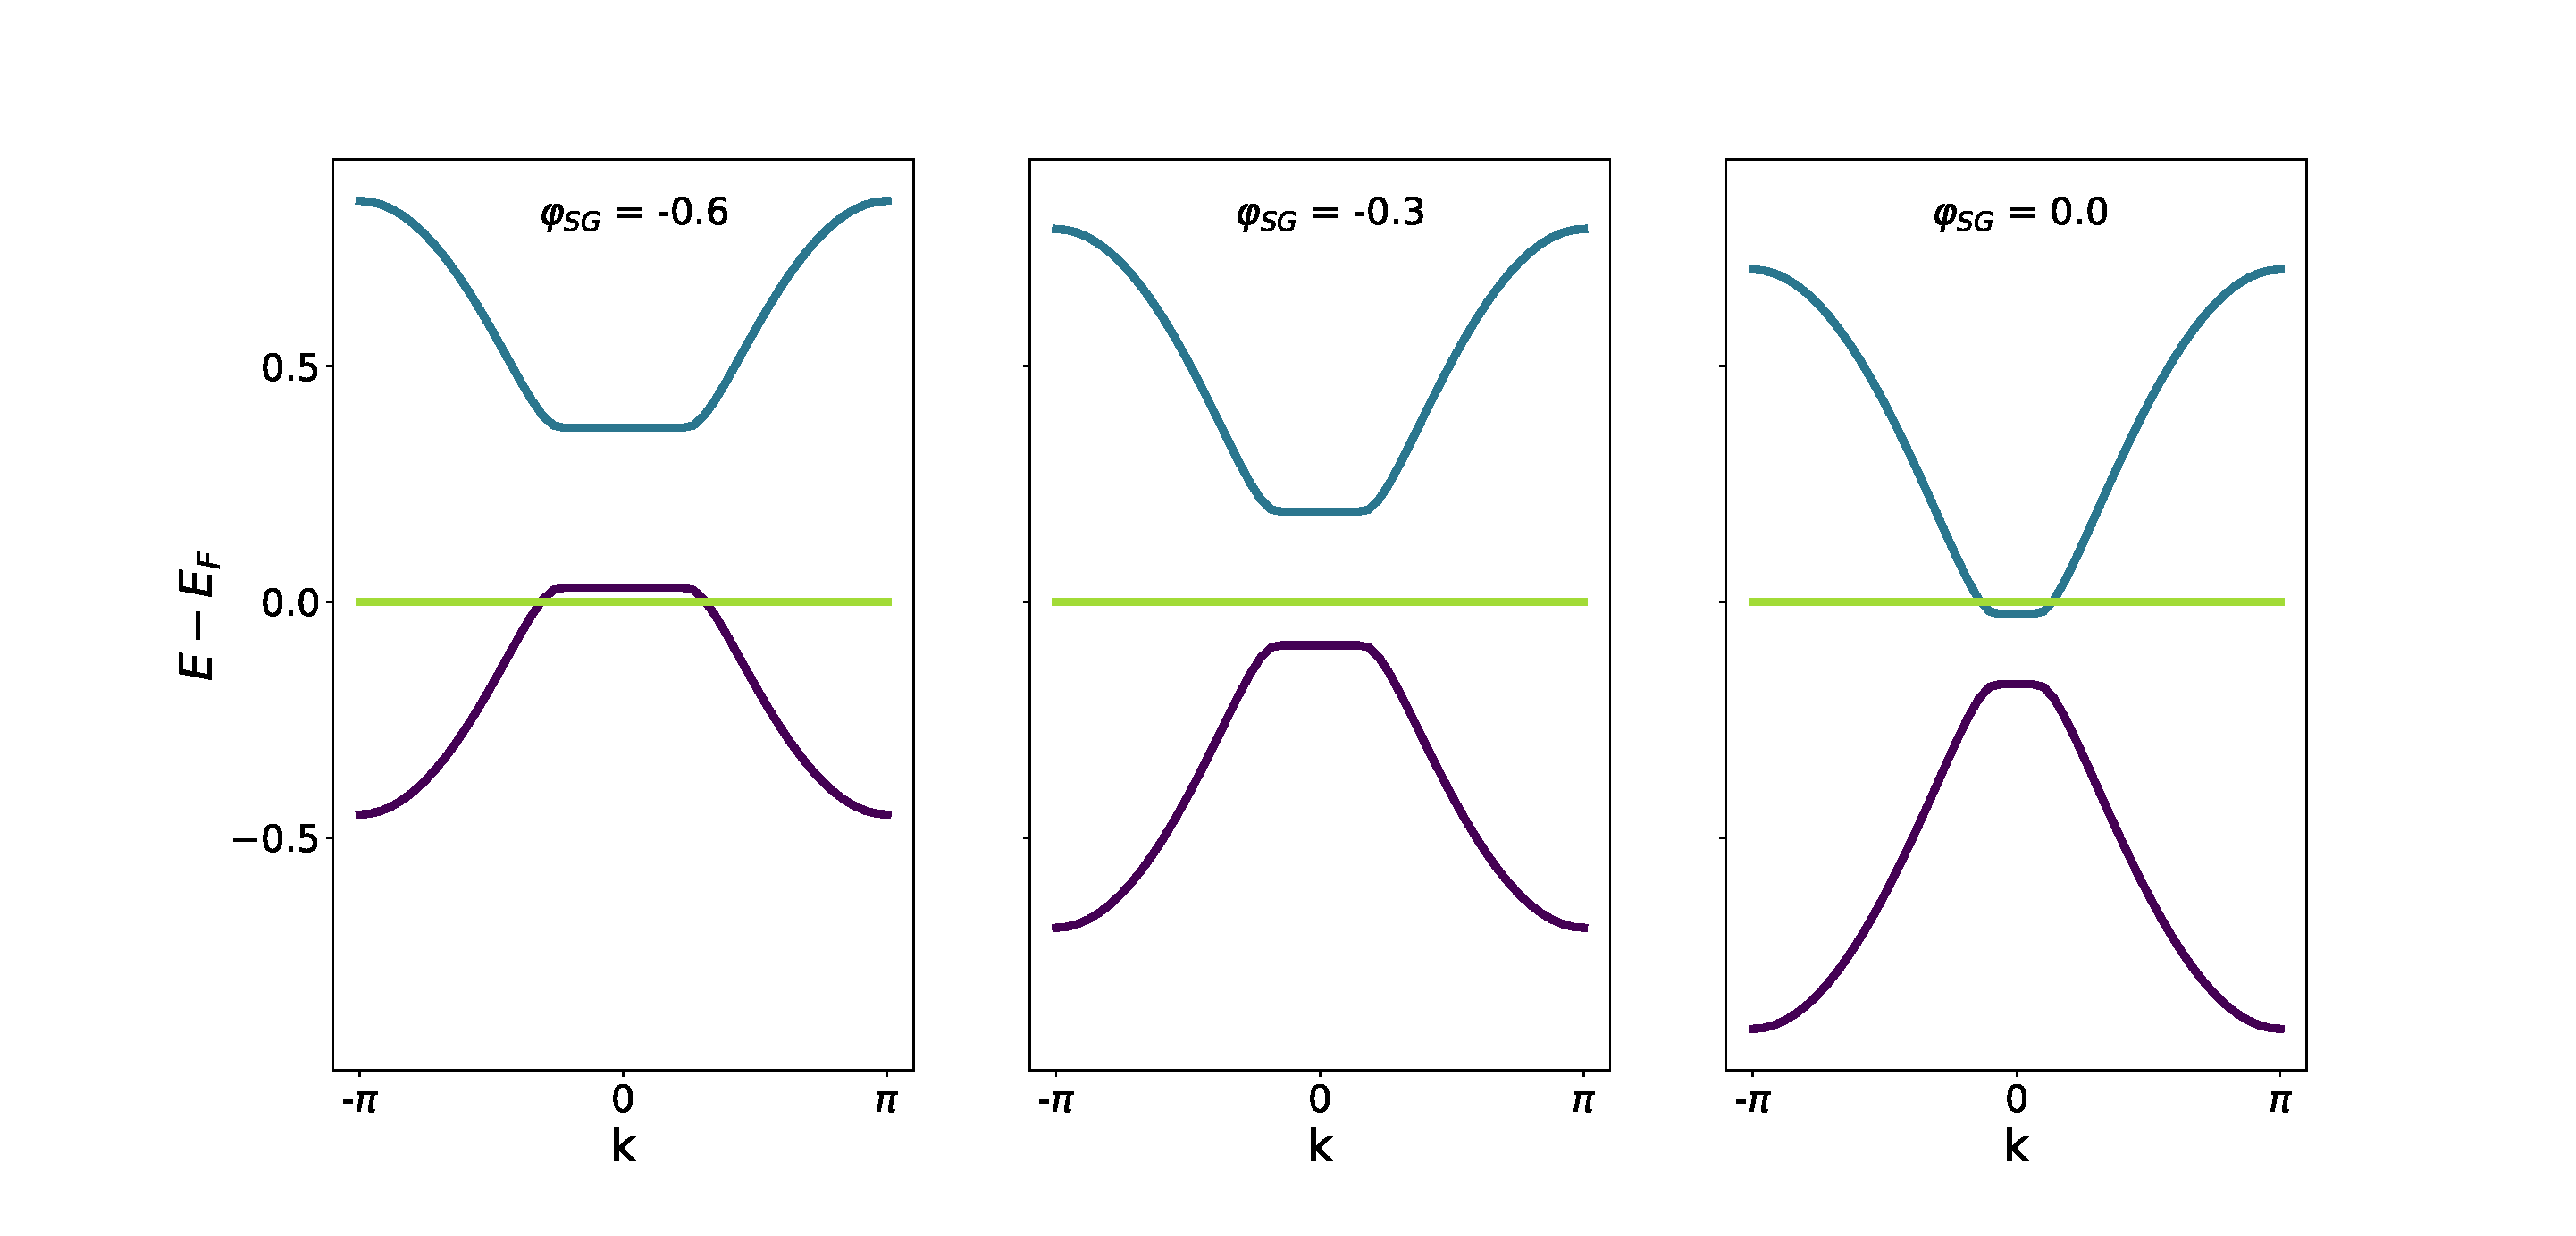
\includegraphics[width=\textwidth]{bands-transition}
\caption{Banstructure for different values of splitgate}
\end{figure}

\section{Waveguide}

Less impact of stray fields

What could be done and has not been evaluated so far:
* impact of disorder in the sample or in the leads
* finite doping in the leads


\section{Half barrier setup}

\begin{figure}
\centering
\begin{minipage}{0.3\textwidth}
\centering
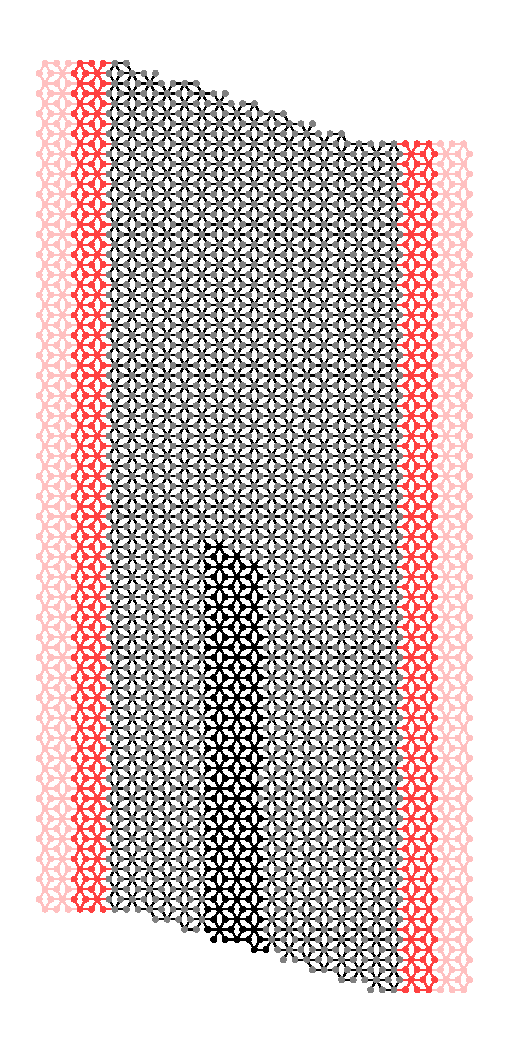
\includegraphics[width=0.6\textwidth]{hb_lower}
\caption{Lower finger}
\end{minipage}%
\begin{minipage}{0.7\textwidth}
\centering
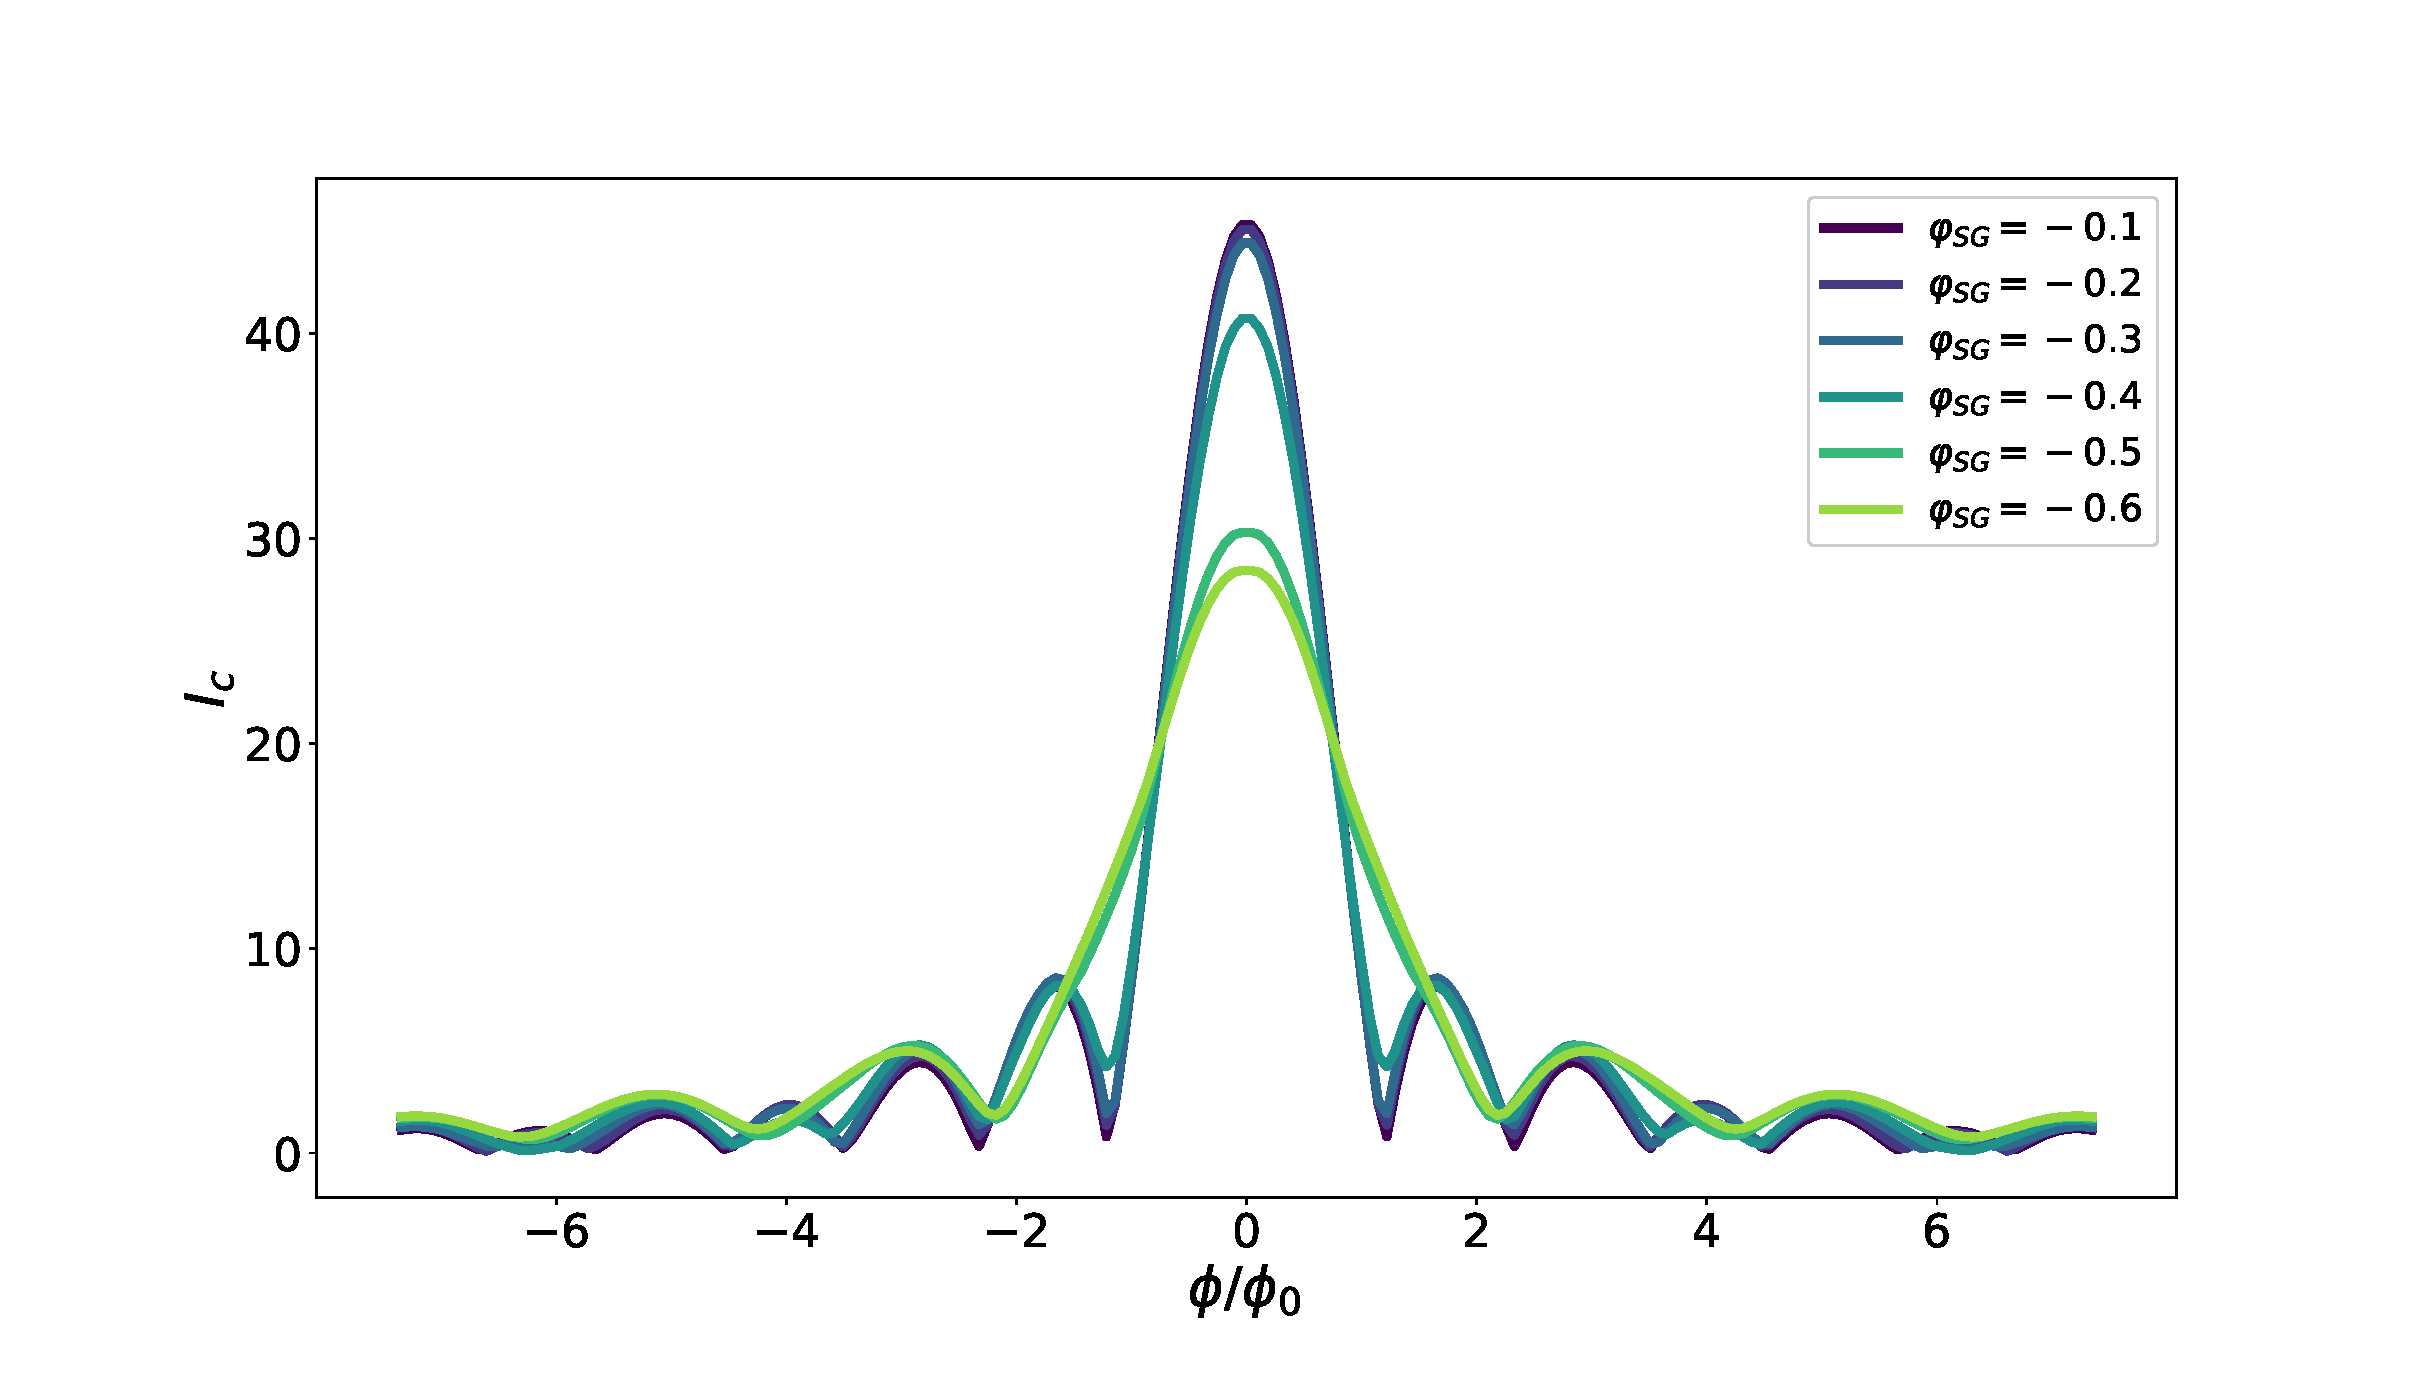
\includegraphics[width=\textwidth]{hb_lower_plot}
\caption{Critical current of lower finger}
\end{minipage}
\end{figure}

\begin{figure}
\centering
\begin{minipage}{0.3\textwidth}
\centering
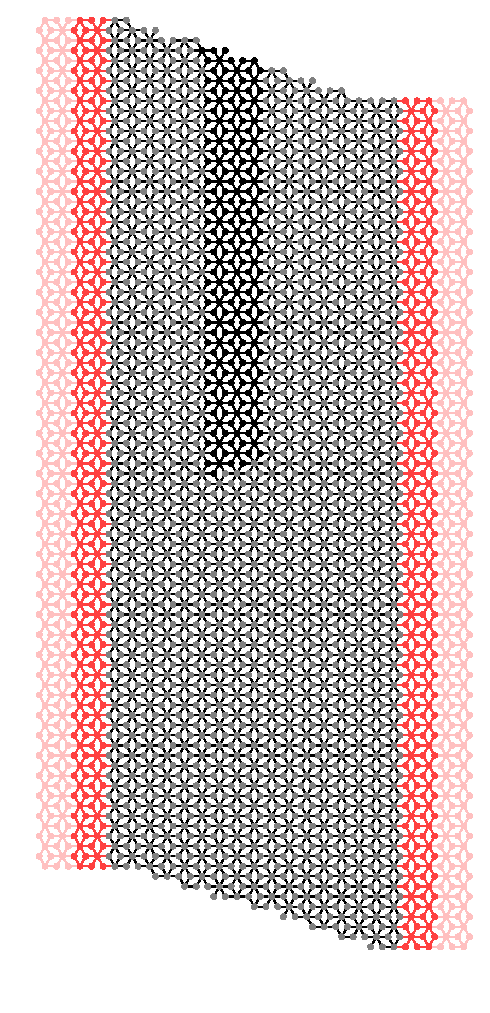
\includegraphics[width=0.6\textwidth]{hb_upper}
\caption{Upper finger}
\end{minipage}%
\begin{minipage}{0.7\textwidth}
\centering
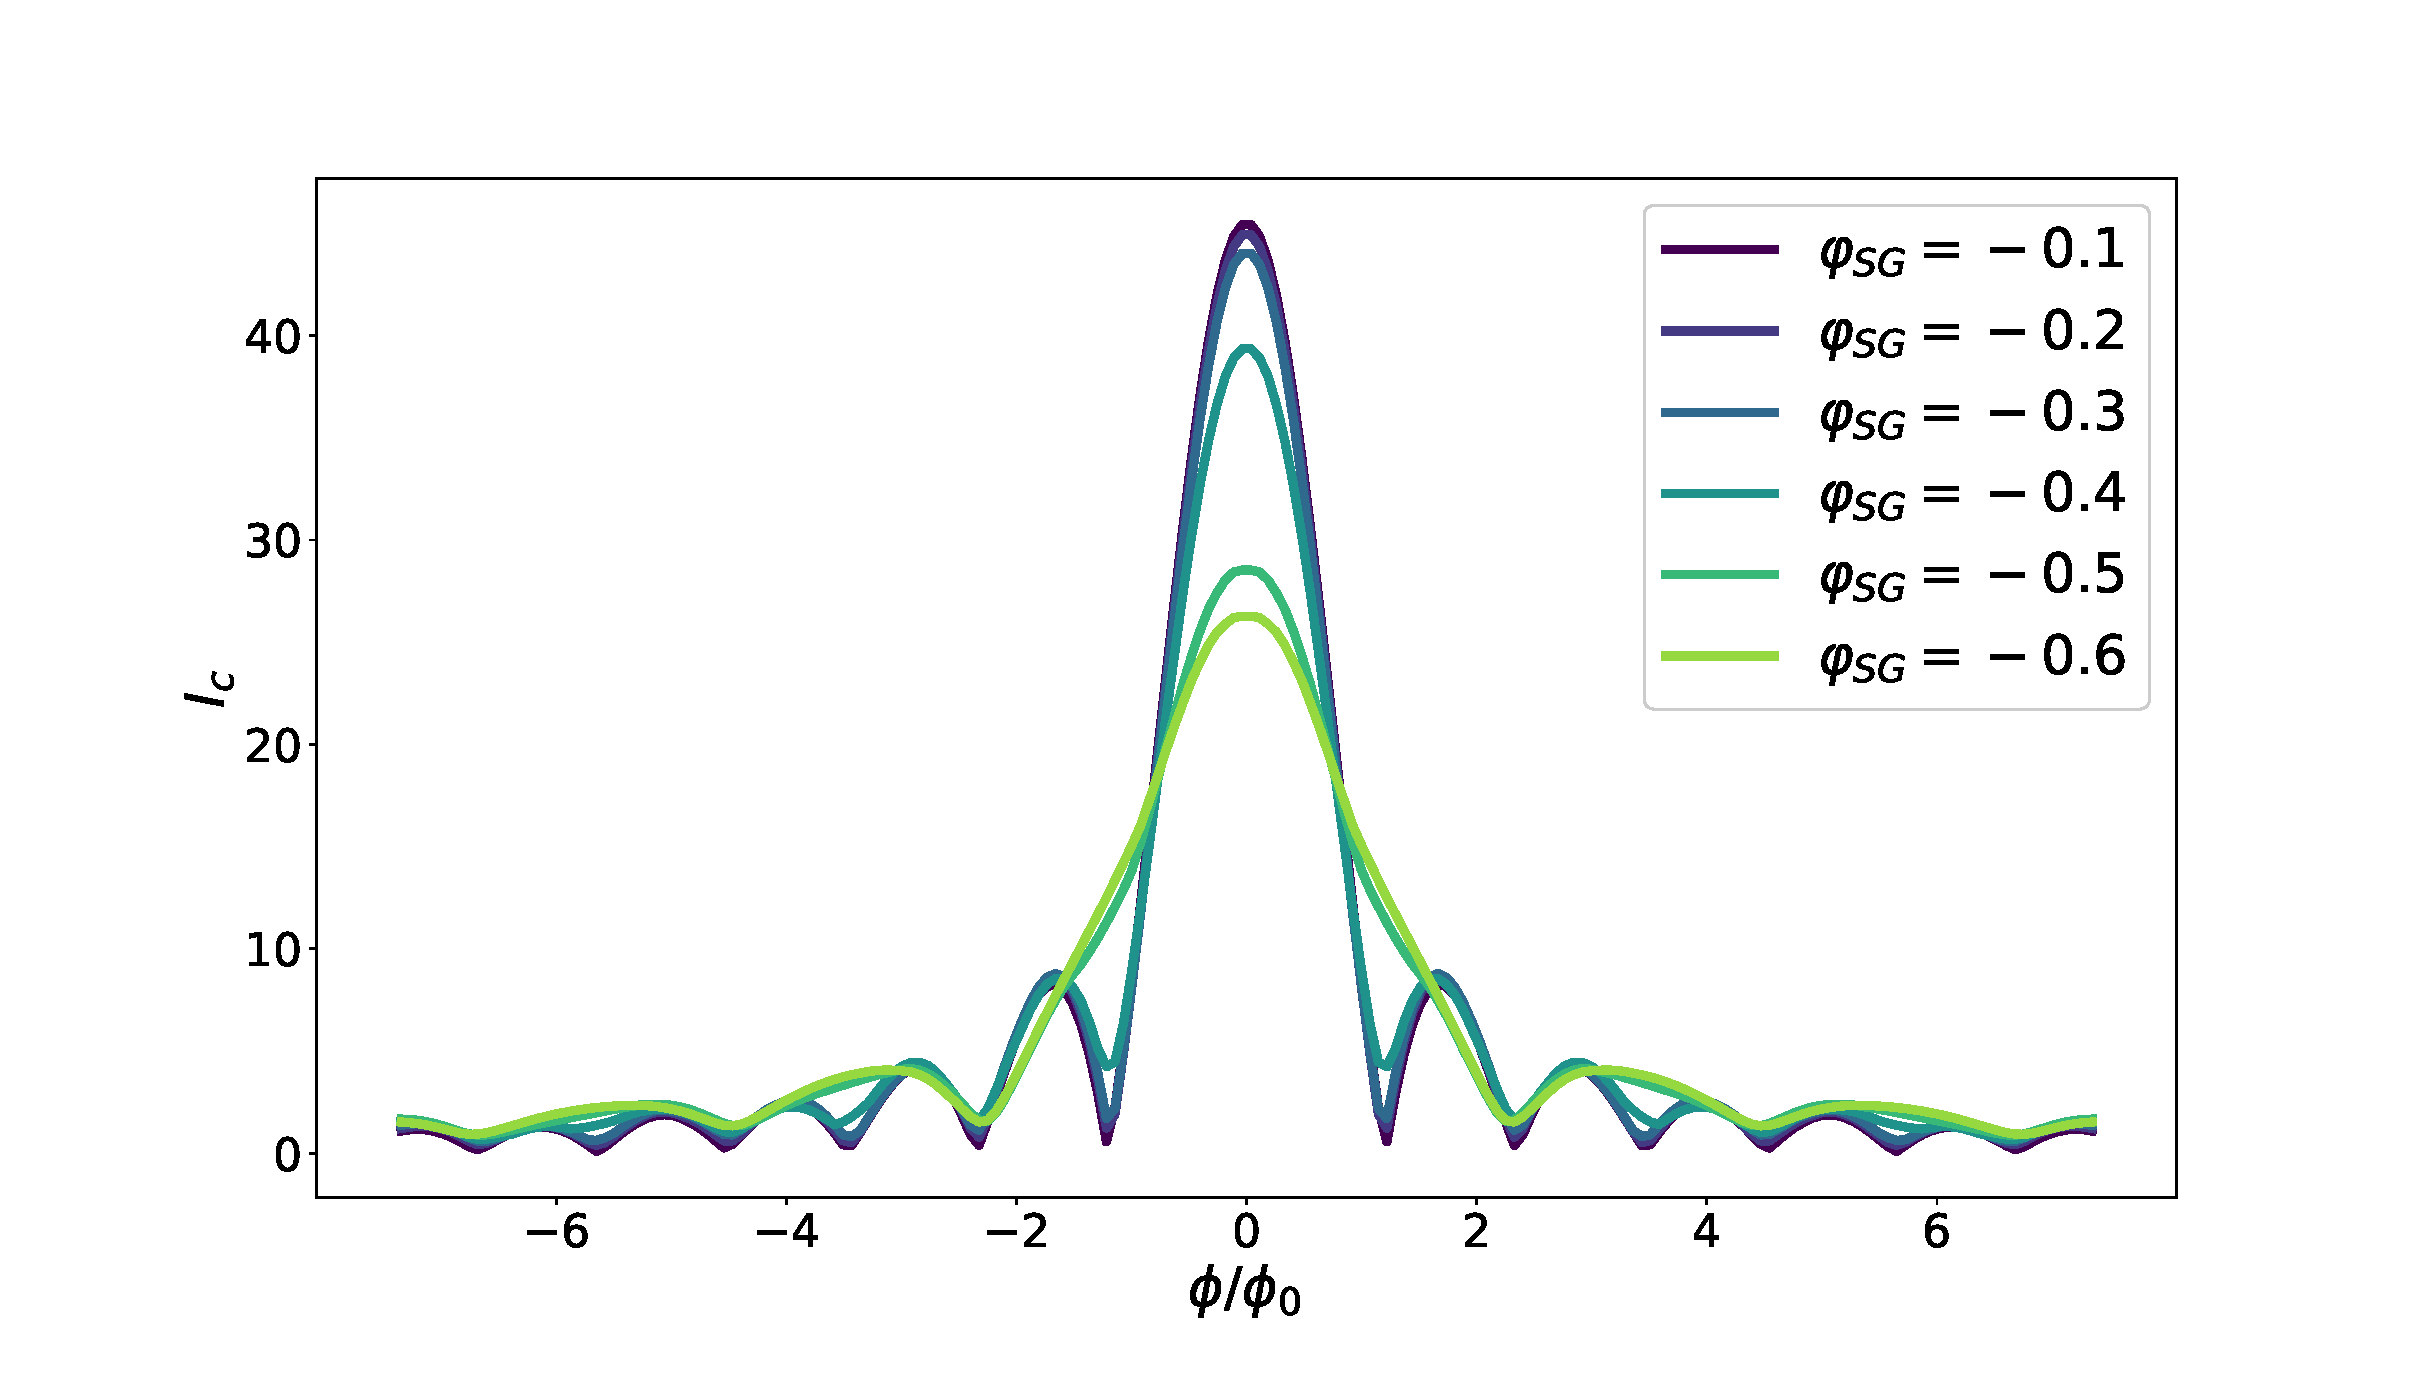
\includegraphics[width=\textwidth]{hb_upper_plot}
\caption{Critical current of upper finger}
\end{minipage}
\end{figure}

\begin{figure}
\centering
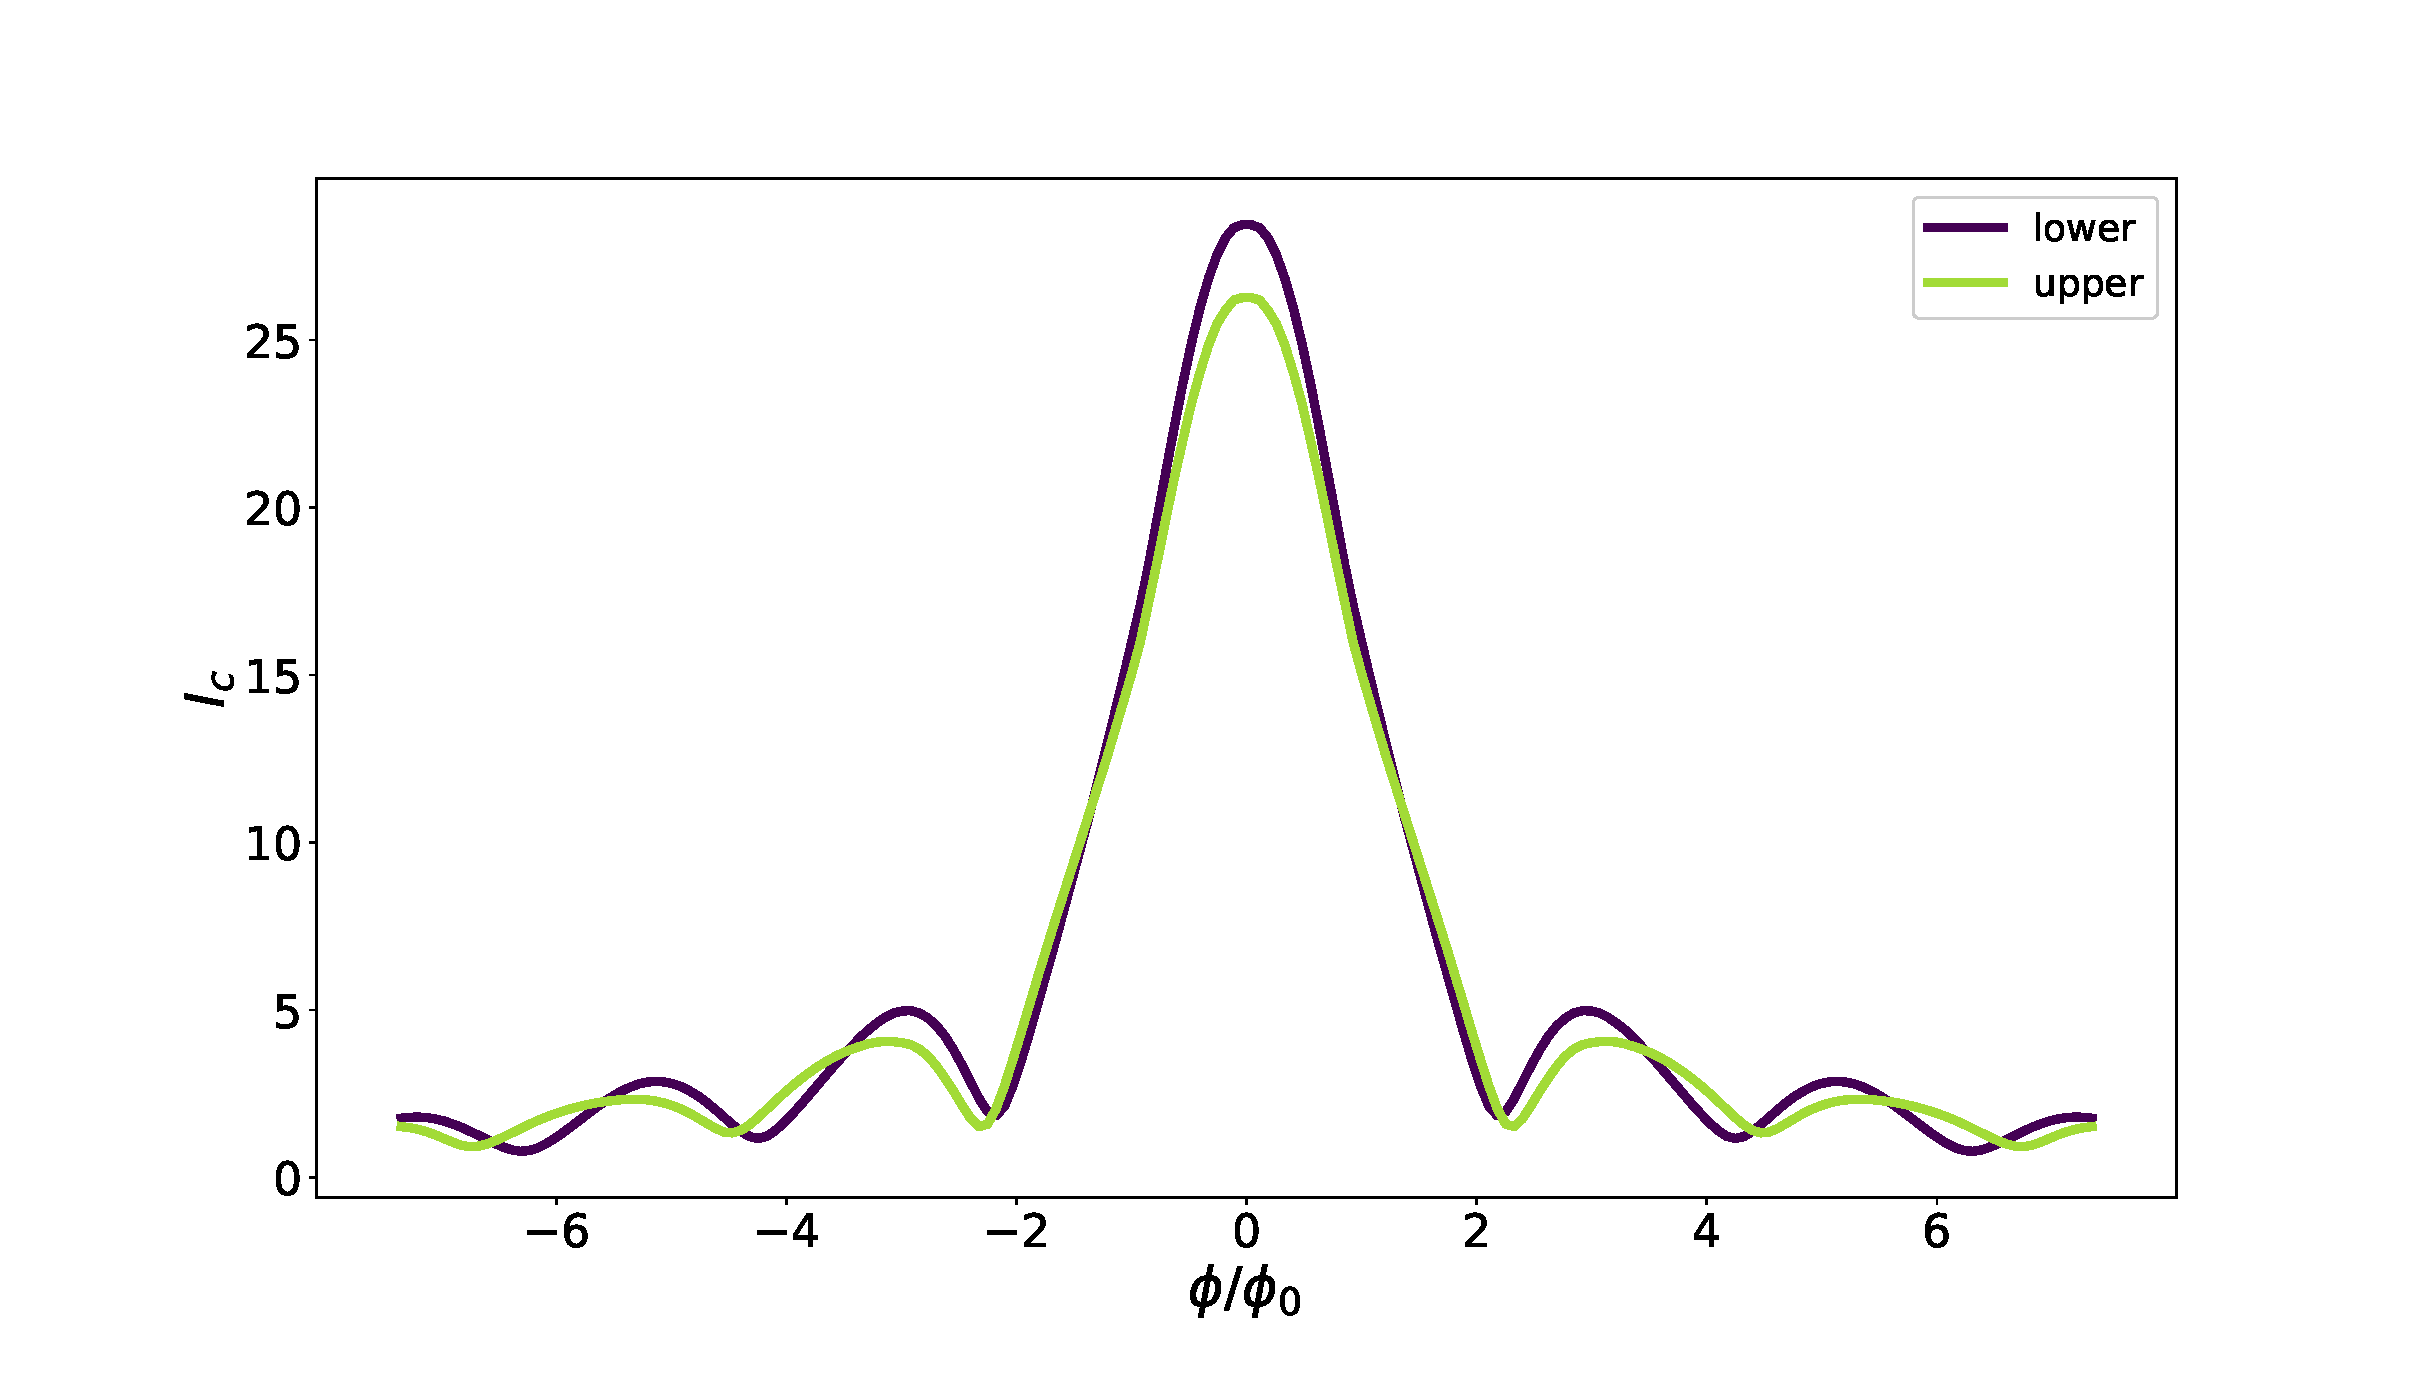
\includegraphics[width=0.8\textwidth]{hb_comparison}
\caption{Comparing critical current curves for upper and lower finger of constriction at the same topgate voltage}
\end{figure}
\end{document}